\clearpage
\graphicspath{{./lib/bob_qkd2/figures/}}
\section{Bob QKD}

\begin{tcolorbox}	
	\begin{tabular}{p{2.75cm} p{0.2cm} p{10.5cm}} 	
        \textbf{Header Files}    &:& bob\_qkd\_*.h \\
		\textbf{Source Files}    &:& bob\_qkd\_*.cpp \\
        \textbf{Version}         &:& 20190410 (Andoni Santos)
	\end{tabular}
\end{tcolorbox}

\maketitle
This block is the main processor for Bob. 

BobQKD is a superblock intended work as Bob's main processor. It performs a 
series of functions, including classical channel communication with Bob and 
data processing for basis reconciliation, error correction and privacy 
amplification.

\subsection*{Input Signals}

\begin{itemize}
	\item[0] - TimeContinuousAmplitudeDiscreteReal signal with received key, to be transmitted to Bob.
	\item[1] - Binary signal with Bob's basis, that will be used to measure the qubits.
	\item[2] - Message signal for receiving incoming messages. 
\end{itemize}

\subsection*{Output Signals}

\begin{itemize}
	\item[0] - Binary signal with Bob's basis, to be used to measure the
	received qubits.
	\item[1] - Binary signal with Bob's final key, after the post processing.
	\item[2] - Message signal for sending outgoing messages.
	\item[3] - (Optional) Binary signal with sifted key.
\end{itemize}

% \subsection*{Signals}

% \begin{table}[h]
% 	\centering
% 	\begin{tabular}{|c|l|}
% 		\hline
% 		\textbf{Number of Input Signals} & 3 \\ \hline
%         \textbf{Type of Input Signals} & Binary,
%         Binary,\\
%         & Message\\\hline
%     	\textbf{Number of Output Signals} & 3 (optionally 4) \ \\ \hline
% 		\textbf{Type of Output Signals} & Binary,Binary,\\
% 		& Message (optional: Binary) \\ \hline
% 	\end{tabular}
% 	\caption{BobQKD signals}
% 	\label{table:bobQKD_signals}
% \end{table}

\subsection*{Input Parameters}


\begin{longtable}{|p{25mm}|p{20mm}|p{20mm}|p{20mm}|p{45mm}|}
	\caption*{\textbf{Note:} all the parameters names are only one word. Some of the parameter's names have been split due to space constraints on the table, but their name is the concatenation of multiple lines shown. This may also be true for some default values.}\label{table:bobQkd_in_par}\\	
	\hline
	\textbf{Parameter} & \textbf{Type} & \textbf{Values} &   \textbf{Default} & \textbf{Description}\\ \hline
	buffSize & unsigned long int & > 0 & 512 & Buffer size for most internal
	signals \\\hline
	maximumEC SyndromeSize & t\_integer & > 0 &  8192 & Buffer size for
	signals where it is important to transmit large quantities of data. \\\hline
	dispBits Interval & t\_integer & > 0 & 50000 & Number of bits transmitted
	before updating the visual interface \\\hline
	folderName & string & valid path & "signals" & Name of the folder where
	signals and output files are saved \\\hline
	reportFile Name & string & valid file name & "bob\_ KeysReport .txt" &
	Name of the file where the overall report for this block is saved
	\\\hline
	toPrint & bool & [true, false] & false & If true, it prints the console
	interface in regular intervals \\\hline
	ipAddress & string & any string & "running locally" & the URL or IP
	address of the remote computer. Only for the purpose of displaying it in the
	interface \\\hline
	% \caption{Error correction input parameters} 
\end{longtable}

\subsection*{Methods}
BobQKD(initializer\_list<Signal *> inputSignals, initializer\_list<Signal *> outputSignals)
\bigbreak
BobQKD(initializer\_list<Signal *> inputSignals, initializer\_list<Signal *> outputSignals, string sFolderName) 
\bigbreak
BobQKD(initializer\_list<Signal*> inputSignals, initializer\_list<Signal*> outputSignals, t\_integer maxSamplesToProcessAtOnce)
\bigbreak
BobQKD(initializer\_list<Signal*> inputSignals, initializer\_list<Signal*> outputSignals, string sFolderName, t\_integer maxSamplesToProcessAtOnce)
\bigbreak
BobQKD(initializer\_list<Signal*> inputSignals, initializer\_list<Signal*> outputSignals, string sFolderName, t\_integer maxSamplesToProcessAtOnce, unsigned long int buffersSize)
\bigbreak
void initialize(void);
\bigbreak
bool runBlock(void);
\bigbreak
bool firstTime{ true };
\bigbreak
void setErrorCorrectionPartitionSize(t\_integer sz)
\bigbreak
void setErrorCorrectionNumberOfPasses(t\_integer np)
\bigbreak
void setDoublePartitionSize(bool db)
\bigbreak
void setMaximumSyndromeSize(t\_integer mss)
\bigbreak
void setMinimumSyndromeSize(t\_integer minss)
\bigbreak
void setDoubleClickNumber(t\_integer dcn)
\bigbreak
void setNoClickNumber(t\_integer ncn)
\bigbreak
void setBer(t\_real berValue)
\bigbreak
void setSystematicSecurityParameter(t\_integer ssp)
\bigbreak
void setBypassHash(bool bh)
\bigbreak
void setMinimumNumberOfPartitions(t\_integer mnp)
\bigbreak
void setParameterEstimationNumberBits(t\_integer nb)
\bigbreak
void setParameterEstimationNumberBitsToStart(t\_integer nbs)
\bigbreak
void setPrint(bool print)
\bigbreak
void setQberThreshold(const t\_real th)
\bigbreak
void setConfidenceInterval(double ci)
\bigbreak
void setIpAddress(string ip)
\bigbreak
string getIpAddress(void)
\bigbreak

\subsection*{Functional description}
\begin{figure}[H]
	\centering
	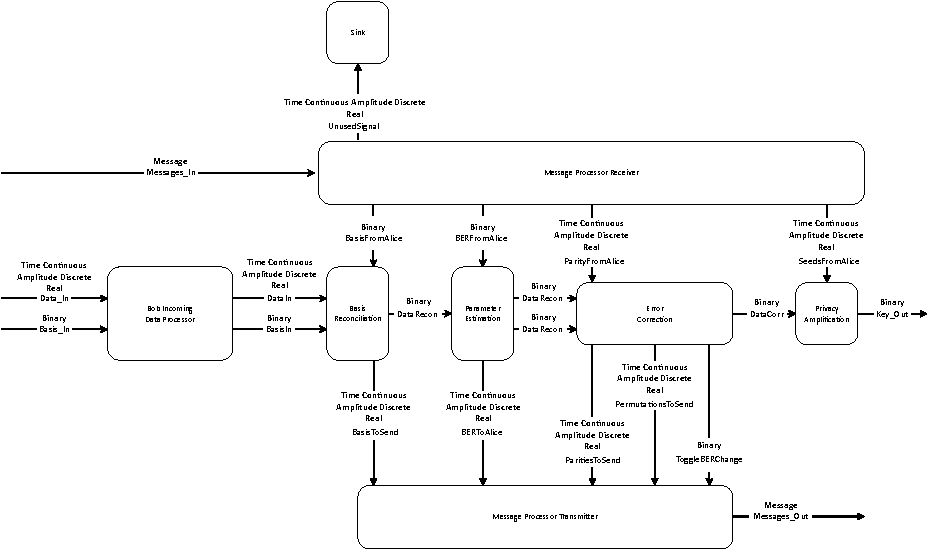
\includegraphics{./lib/bob_qkd2/figures/blockDiagram_bob.pdf}
\end{figure}

BobQKD is a superblock intended to do classical channel communication and 
data processing  as required by the BB84 protocol. This superblock requires 
four different inputs:

\begin{itemize}
	\item Messages from Alice, which are used to coordinate the required data 
	processing for key extraction;
	\item A binary signal corresponding to the measured transmitted data;
	\item A binary signal corresponding to the basis used by Bob for 
	decoding the data sent by Alice.
\end{itemize}

In addition, this block can produce a total of four output signals:

\begin{itemize}
	\item A binary signal with Bob's basis;
	\item A binary signal with the generated key;
	\item Messages intended to be read by Alice, used to coordinate the required 
	data processing for key extraction;
	\item An optional signal with the sifted key.
\end{itemize}

% The process inside the superblock is as follows:

The incoming data and basis signals are received in the 
\textit{BobIncomingDataProcessor} block. If the transmission is enabled, the 
incoming data and basis are sent into the \textit{BasisReconciliation} block.

The \textit{BasisReconciliation} block in BobQKD is configured to start the
basis reconciliation process, as opposed to AliceQKD which waits for Bob to
receive information first in order to respond. Thus, when enough samples are available, Bob
sends a signal with the list of used basis to the 
\textit{MessageProcessorTransmitter} block. The block then waits.
When Alice responds, a message arrives at the \textit{MessageProcessorReceiver} 
block. It contains a binary string indicating whether Bob used the correct 
basis or not. This information is then sent to the \textit{BasisReconciliation} 
block. There, the bits where Bob got the right basis are sent to the 
\textit{ParameterEstimation} block, while the remaining ones are promptly discarded.

The \textit{ParameterEstimation} block is the next one to be active. Here, the
sifted key will be accumulated until its size is large enough, as defined by the
method \textit{setParameterEstimationNumberBitsToStart}. Once this happens, the
block will use a seeded pseudorandom number generator to select a predefined number of
samples from the accumulated key. It then sends Alice a message containing the
seed and the sampled value, so she can compare with the results she has. She
eventually sends a response with how Bob's values compare to hers. The ratio of
wrong values provides an estimate for the QBER. If the QBER estimate upper bound is higher
than a given threshold, all the stored values in the interval are discarded, as
it means that they can't be trusted. Otherwise, the sampled values are then
discarded, and the remaining ones are sent to the \textit{ErrorCorrection}
block, along with the QBER estimate.

The \textit{ErrorCorrection} block will be responsible for correcting any 
errors that occurred during transmission. Similarly to the 
\textit{BasisReconciliation} block, in BobQKD it is configured to start acting 
when enough samples are available. When this condition is verified, the 
\textit{ErrorCorrection} block starts the Cascade process by dividing the 
available bits in segments, calculating their parities and sending them to the 
\textit{MessageProcessorTransmitter}. Once this is done, it waits until a 
response from Alice arrives at \textit{MessageProcessorReceiver}. The message 
should contain a response to Bob on whether the parities are similar or not. The 
Cascade process continues until it is concluded. The Cascade process is 
explained in the section of the \textit{ErrorCorrection} block, but is not 
fundamental to understanding the BobQKD superblock.

When the cascade process ends, the corrected data is output to the 
\textit{PrivacyAmplification} block, which does the necessary transformation to 
ensure the information that any attacker might have gained (Eve) is nullified.

The end result, and final output of the superblock, is a secure key 
shared known only to Alice and Bob.


\subsection*{Examples}


\subsection*{Sugestions for future improvement} 



%%%%%%%%%%%%%%%%%%%%%%%%%%%%%%%%%%%%%%%%%%


% \subsection*{Signals}

% \begin{table}[h]
% 	\centering
% 	\begin{tabular}{|c|l|}
% 		\hline
% 		\textbf{Number of Input Signals} & 3 \\ \hline
%         \textbf{Type of Input Signals} & Binary,
%         Binary,\\
%         & Message\\\hline
%     	\textbf{Number of Output Signals} & 5 \ \\ \hline
% 		\textbf{Type of Output Signals} & Binary,Binary,Binary,\\
% 		& Message,Binary \\ \hline
% 	\end{tabular}
% 	\caption{AliceQKD signals}
% 	\label{table:bin_sour_signals}
% \end{table}

% \subsection*{Input Parameters}

% \begin{longtable}{|p{25mm}|p{20mm}|p{20mm}|p{20mm}|p{45mm}|}
% 	\caption*{\textbf{Note:} all the parameters names are only one word. Some of the parameter's names have been split due to space constraints on the table, but their name is the concatenation of multiple lines shown. This may also be true for some default values.}\label{table:aliceQkd_in_par}\\	
% 	\hline
% 	\textbf{Parameter} & \textbf{Type} & \textbf{Values} &   \textbf{Default} & \textbf{Description}\\ \hline
% 	buffSize & unsigned long int & > 0 & 512 & Buffer size for most internal
% 	signals \\\hline
% 	maximumEC SyndromeSize & t\_integer & > 0 &  8192 & Buffer size for
% 	signals where it is important to transmit large quantities of data. \\\hline
% 	dispBits Interval & t\_integer & > 0 & 50000 & Number of bits transmitted
% 	before updating the visual interface \\\hline
% 	folderName & string & valid path & "signals" & Name of the folder where
% 	signals and output files are saved \\\hline
% 	reportFile Name & string & valid file name & "alice\_ KeysReport .txt" &
% 	Name of the file where the overall report for this block is saved
% 	\\\hline
% 	toPrint & bool & [true, false] & true & If true, it prints the console
% 	interface in regular intervals \\\hline
% 	ipAddress & string & any string & "running locally" & the URL or IP
% 	address of the remote computer. Only for the purpose of displaying it in the
% 	interface \\\hline
% 	photonsPer Pulse & double & any & 0.1 & Average number of photons sent in
% 	each transmitted pulse. Only for the purpose of displaying it in the
% 	interface. \\\hline
% 	% \caption{Error correction input parameters} 
% \end{longtable}



% \subsection*{Methods}
% void initialize(void)
% \bigbreak
% bool runBlock(void)
% \bigbreak
% AliceQKD(initializer\_list<Signal *> inputSignals, initializer\_list<Signal *> outputSignals)
% \bigbreak
% AliceQKD(initializer\_list<Signal*> inputSignals, initializer\_list<Signal*> outputSignals, string sFolderName)
% \bigbreak
% AliceQKD(initializer\_list<Signal*> inputSignals, initializer\_list<Signal*> outputSignals, t\_integer maxSamplesToProcessAtOnce)
% \bigbreak
% AliceQKD(initializer\_list<Signal*> inputSignals, initializer\_list<Signal*> outputSignals, string sFolderName, t\_integer maxSamplesToProcessAtOnce)
% \bigbreak
% AliceQKD(initializer\_list<Signal*> inputSignals, initializer\_list<Signal*> outputSignals, string sFolderName, t\_integer maxSamplesToProcessAtOnce, unsigned long int buffersSize)
% \bigbreak
% void setErrorCorrectionPartitionSize(t\_integer sz)
% \bigbreak
% void setErrorCorrectionNumberOfPasses(t\_integer np)
% \bigbreak
% void setDoublePartitionSize(bool db)
% \bigbreak
% void setMaximumSyndromeSize(t\_integer mss)
% \bigbreak
% void setMinimumSyndromeSize(t\_integer minss)
% \bigbreak
% void setDoubleClickNumber(t\_integer dcn)
% \bigbreak
% void setNoClickNumber(t\_integer ncn)
% \bigbreak
% void setBer(t\_real berValue)
% \bigbreak
% void setSystematicSecurityParameter(t\_integer ssp)
% \bigbreak
% void setBypassHash(bool bh)
% \bigbreak
% void setMinimumNumberOfPartitions(t\_integer mnp)
% \bigbreak
% void setParameterEstimationNumberBits(t\_integer nb)
% \bigbreak
% void setParameterEstimationNumberBitsToStart(t\_integer nbs)
% \bigbreak
% void setPrint(bool print)
% \bigbreak
% void setQberThreshold(const t\_real th)
% \bigbreak
% void setPhotonsPerPulse(double ppp)
% \bigbreak
% void setConfidenceInterval(double ci)
% \bigbreak
% void setIpAddress(string ip)
% \bigbreak
% string getIpAddress(void)


% \subsection*{Functional description}

% \begin{figure}[H]
% 	\centering
% 	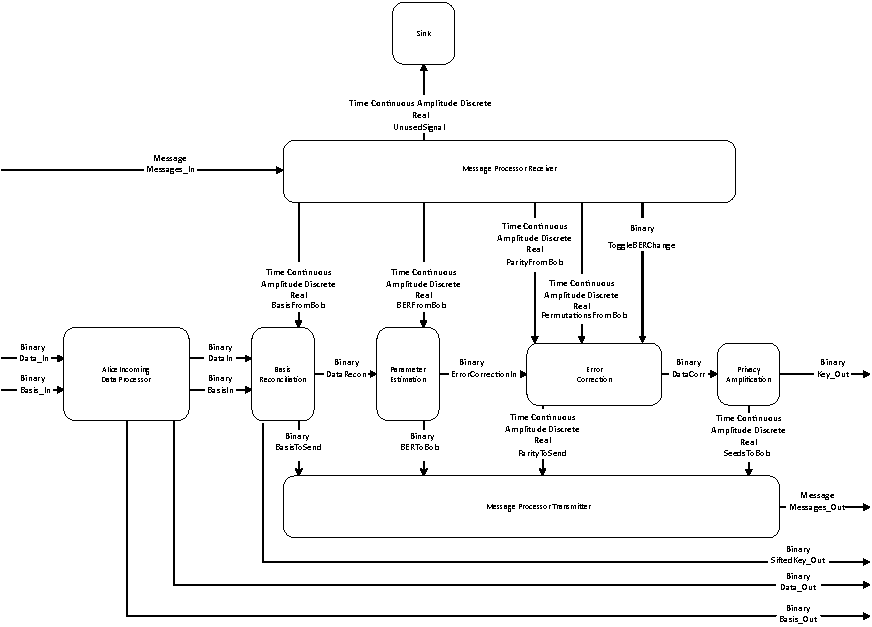
\includegraphics{./lib/alice_qkd2/figures/AliceQKD_blockDiagram.pdf}
% \end{figure}

% AliceQKD is a superblock intended to do classical channel communication and 
% data processing  as required by the BB84 protocol. This superblock requires 
% three different inputs:

% \begin{itemize}
% 	\item Messages from Bob, which are used to coordinate the required data 
% 	processing for key extraction;
% 	\item A binary signal to be used for the transmitted key;
% 	\item A binary signal corresponding to the basis which will be used for 
% 	encoding the data.
% \end{itemize}

% In addition, this block produces a total of four (or five, optionally) output signals:

% \begin{itemize}
% 	\item	Messages intended to be read by Bob, used to coordinate the required 
% 	data processing for key extraction;
% 	\item A binary signal of the data, to be transmitted through the quantum 
% 	channel;
% 	\item A binary signal corresponding to the basis which will be used to 
% 	encoded the transmitted data;
% 	\item A binary signal with the generated key;
% 	\item An optional binary signal corresponding to the sifted key.
% \end{itemize}


% The process inside the superblock is as follows:

% The incoming data and basis binary signals are provided as inputs to the 
% \textit{AliceIncomingDataProcessor}, together with the 
% \textit{transmissionMode} signal. 
% The transmission mode controls the behaviour of the 
% \textit{AliceIncomingDataProcessor}: it either enables it to continue working 
% or tells it to stop reading the input data, while it waits for the current data
% to be dispatched.
% The data and basis read at the block are sent twice each to the output signals, 
% keeping their sync. Each pair of basis and data has a different destination: 
% one of the pair is directed to the superblock outputs, in order to transmit the 
% data and control the basis for the transmission; and the other pair is sent to 
% the \textit{BasisReconciliation} block.

% The \textit{BasisReconciliation} block in AliceQKD is configured to responding
% to Bobs messages, instead of sending them first. Therefore, it now waits for a 
% signal from the 
% \textit{MessageProcessorReceiver}. When Bob has enough samples, he should send 
% a message containing the basis he used to measure the received data. This 
% message is received, identified by its type \texttt{BasisReconciliation1}, and 
% interpreted at the \textit{MessageProcessorReceiver}. 
% When a message of the correct type arrives, this block sends a signal to the 
% \textit{BasisReconcilliation} block, containing the list of basis Bob used to 
% measure the data on his side. The \textit{BasisReconciliation} block then 
% compares the basis received from Bob with the ones that Alice used, and based 
% on this is outputs two signals:

% \begin{itemize}
% 	\item A binary evaluation of which basis used 
% 	by Bob are correct. This is sent to the \textit{MessageProcessorTransmitter}, 
% 	so that a message can be sent to Bob for him to know which basis were correct.
% 	\item A binary signal containing the data sent when those basis were used. 
% 	This is the data that Bob should have measured correctly. This signal is sent 
% 	to the \textit{ErrorCorrection} block.
% \end{itemize} 

% The \textit{ErrorCorrection} block will be responsible for correcting any 
% errors that occurred during transmission. Similarly to the 
% \textit{BasisReconciliation} block, it is configured to act in response to Bobs 
% messages. As such, it waits for data from the 
% \textit{MessageProcessorReceiver}, and outputs a response to the 
% \textit{MessageProcessorTransmitter}. It also outputs a copy of the 
% signal from basis reconciliation, after it has been used for error correction. 
% This is will be the transmitted key, free from errors.


% When the \textit{MessageProcessorReceiver} receives a message with the type 
% \texttt{ErrorCorrection1}, it starts the Cascade error correction process.
% That message contains the necessary information used in the Cascade process. 
% The explanation of the whole error correction process is somewhat long and not 
% required to understand how the AliceQKD block works. Therefore, further details 
% can be found in the \textit{ErrorCorrection} block's documentation.

% After each set of bits is corrected, the data is output to the 
% \textit{PrivacyAmplification} block, which does the necessary transformation to 
% ensure the information that any attacker might have gained (Eve) is nullified.

% The end result, and final output of the superblock, is a secure key 
% shared known only to Alice and Bob.

% \subsection*{Examples}

% \subsection*{Suggestions for future improvement}